% !TEX root = /Users/zhuzhuangdi/Desktop/MSUCourses/MachineLearning847/17Project/17spr_wang_zhu_du/Middle/middle_report.tex
\section{Project Milestones} 

\subsection{Completed Milestones} 
\judy{To be re-written}
%
\subsubsection{Background Survey}
 For this initial step, we plan to search for related works to computational literary creation to gain the basic knowledge of Song Ci.
%
We are interested in the following questions: what is the criterion of a good Song Ci? How to evaluate the correctness, fluency and style of poems generated?
%
Better understanding of related work and Song Ci composition rules will provide us with great help for the following work, especially algorithm testing and comparison. 
%
\subsubsection {Corpus Search and Analysis}
%
Second, we will search and select a proper Song poem corpus for our project. The ideal corpus should be comprehensive on poem styles, and are precisely analyzed for content. 
%
\subsubsection{ Implementation of Vector Space Model }
Test cases will be generated with both poem generator under the same keywords and topics. Poems will be test on aspects of grammar, semantic correctness, style and content. Both computational evaluation and human evaluation are expected to be used in last part of our project.
\subsubsection{ Implementation of RNN + SLTM Model  }   
Third, implementation poem generator based on both algorithm of RNN and genetic algorithm would be the most important work in our project. So we will assign more time on this step. 
%

\subsection{Remaining Milestones}


\begin{itemize}
\item Implementation of Genetic Algorithms 
\item Model Testing and Comparison
\item Project Summary and Writing
\end{itemize}

\begin{figure}[htbp]
	\centering
	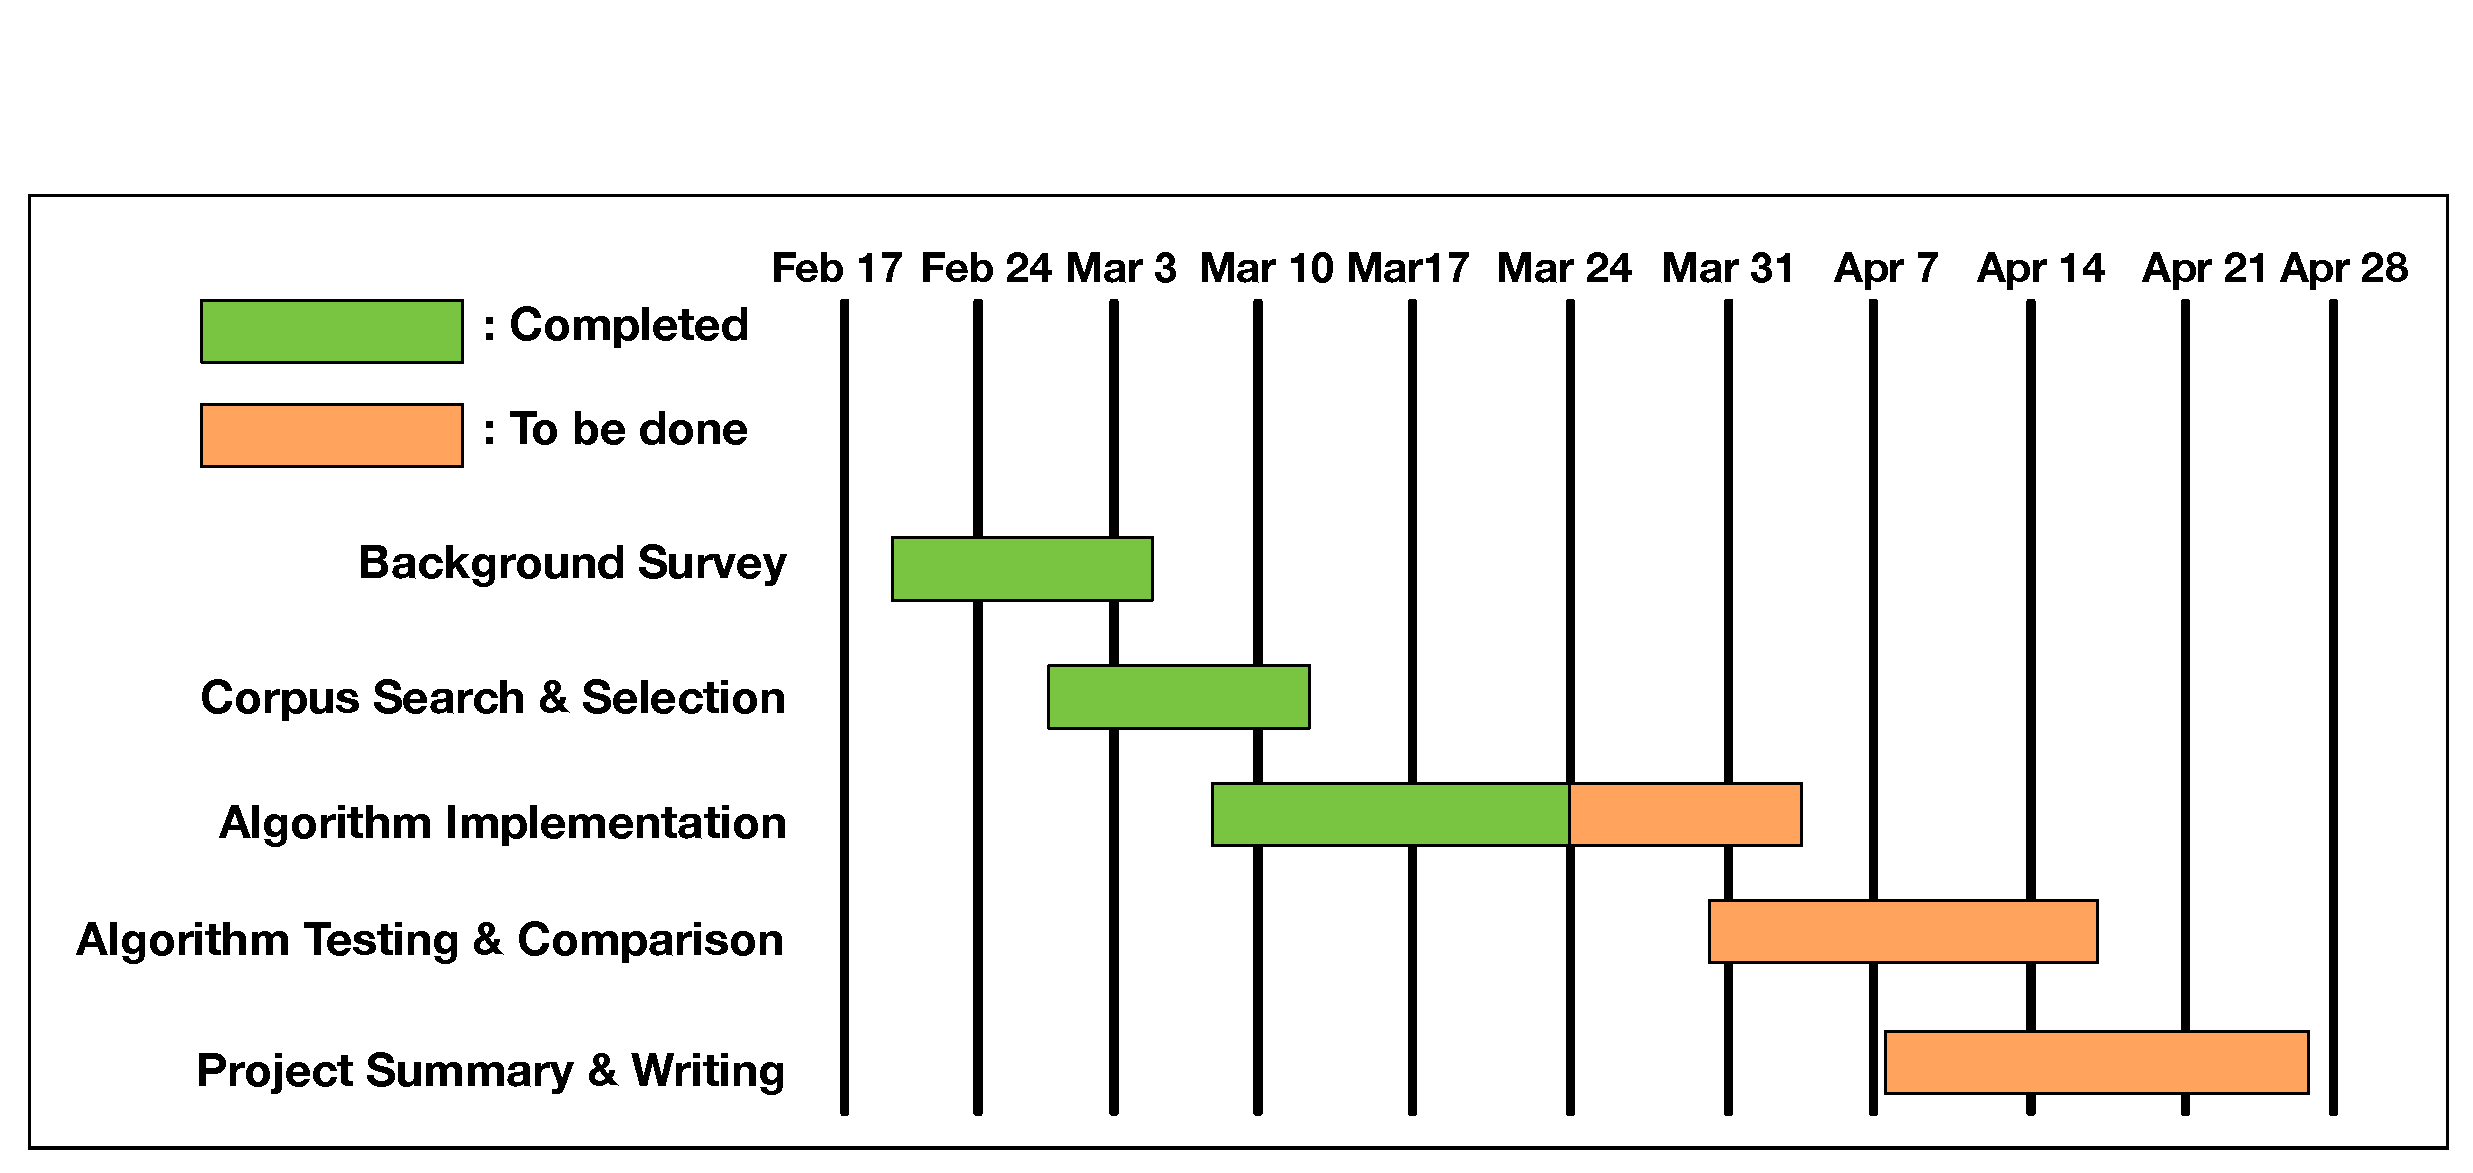
\includegraphics[width=0.9\linewidth]{mileStone}
	\caption{Project Timeline}
	\label{fig:projecttimeline}	
\end{figure} 